\section[Vorlesung 1: Modellierung von (dynamischen) Systemen und\\ Prozessen]{Vorlesung 1: Modellierung von (dynamischen) Systemen und Prozessen}
\markright{Vorlesung 1: Modellierung von (dynamischen) Systemen und Prozessen}

\subsection*{Grundlegende Elemente der Verhaltensmodellierung}

Eine Modellierungssprache legt fest, 
\marginline{Syntax und Semantik der Modellierungs\-sprache}
welche Elemente zur Beschreibung eines Originals genutzt und wie sie dargestellt werden. Ähnlich wie in einer natürlichen Sprache gibt es dabei eine Syntax: Formale Regeln bestimmen, welche Symbole zur Darstellung der verschiedenen Elemente verwendet werden und wie sie kombiniert werden können. Die Semantik hingegen definiert die Bedeutungen dieser Symbole. Sie bestimmt also, \textbf{wie} Originale abgebildet werden und damit auch, welche ihrer Aspekte durch die jeweilige Modellierungssprache hervorgehoben werden. Ein Element kann in verschiedenen Modellierungssprachen unterschiedlich benannt und durch unterschiedliche Symbole repräsentiert werden \cite{ros12}.

Unterschiede ergeben sich aus dem jeweiligen Modellierungskontext und -zweck. Die Abbildungen \ref{fig:grundelemente_EPK} und \ref{fig:grundelemente_BPMN} zeigen als Beispiele die zwei heute gängigen Prozess\-model\-lie\-rungs\-sprachen EPK und BPMN (im Vorlesungsvideo werden weitere Sprachen vorgestellt).

\begin{figure}[t]
	\begin{addmargin*}[0cm]{-\marginparwidth}
	\begin{addmargin*}[0cm]{-\marginparsep}
		\centering
		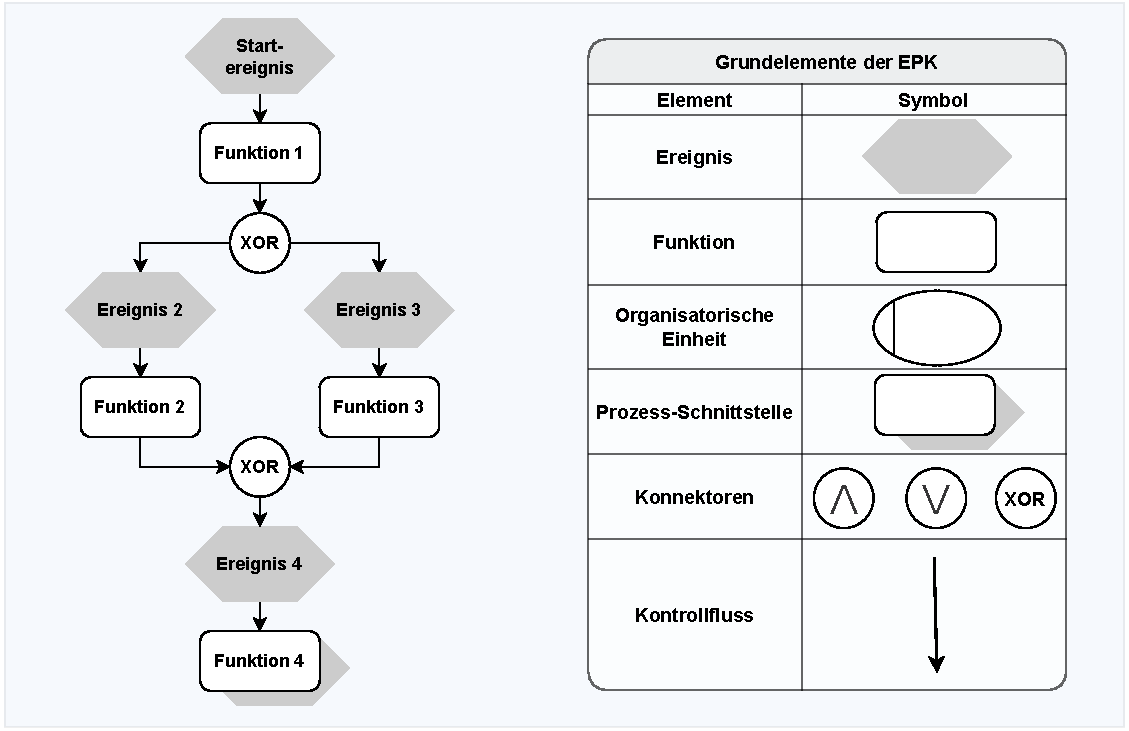
\includegraphics[scale=0.9]{Bilder/Kapitel-5/grundelemente_EPK.pdf}
		\caption{EPK}
		\label{fig:grundelemente_EPK}
	\end{addmargin*}
	\end{addmargin*}
\end{figure}

Abbildung~\ref{fig:grundelemente_EPK} zeigt eine ereignisgesteuerte Prozesskette (EPK) 
\marginline{Beispiel: EPK}
und ihre typischen Elemente und Symbole. EPKs wurden in den 1990er Jahren zur Modellierung von Geschäftsprozessen von Organisationen entwickelt \cite{kel92}. In EPKs gibt es, wie in vielen Prozessmodellierungssprachen, Aktivitäten (hier Funktionen genannt) und lokale Zustände (hier Ereignisse genannt) sowie die Konnektoren UND, ODER und exklusives ODER (XOR), die mögliche Abläufe und ihre Verzweigungen definieren. Es existieren in EPKs weitere Elemente wie Rollen oder notwendige Ressourcen.

Im Kontext der Prozessmodellierung wird das Wort „Ereignis“ leider auf unterschiedliche Weise verwendet. Was hier als „Ereignis“ bezeichnet wird, heißt in anderen Modellierungssprachen als „Bedingung“ oder „lokaler Zustand“.

Etwas moderner als die EPKs sind 
\marginline{Beispiel: BPMN}
Business Process Model and Notation (BPMN)-Diagramme. Diese Modellierungssprache entstand Anfang der 2000er Jahre bei IBM und wird seit 2005 von der Object Management Group (OMG) verwaltet, die auch für die Unified Modeling Language (UML) verantwortlich ist \cite{wes24}. Abbildung~\ref{fig:grundelemente_BPMN} zeigt ein BPMN-Diagramm mit seinen typischen Elementen und Symbolen.

\begin{figure}[!htbp]
	\begin{addmargin*}[0cm]{-\marginparwidth}
	\begin{addmargin*}[0cm]{-\marginparsep}
		\centering
		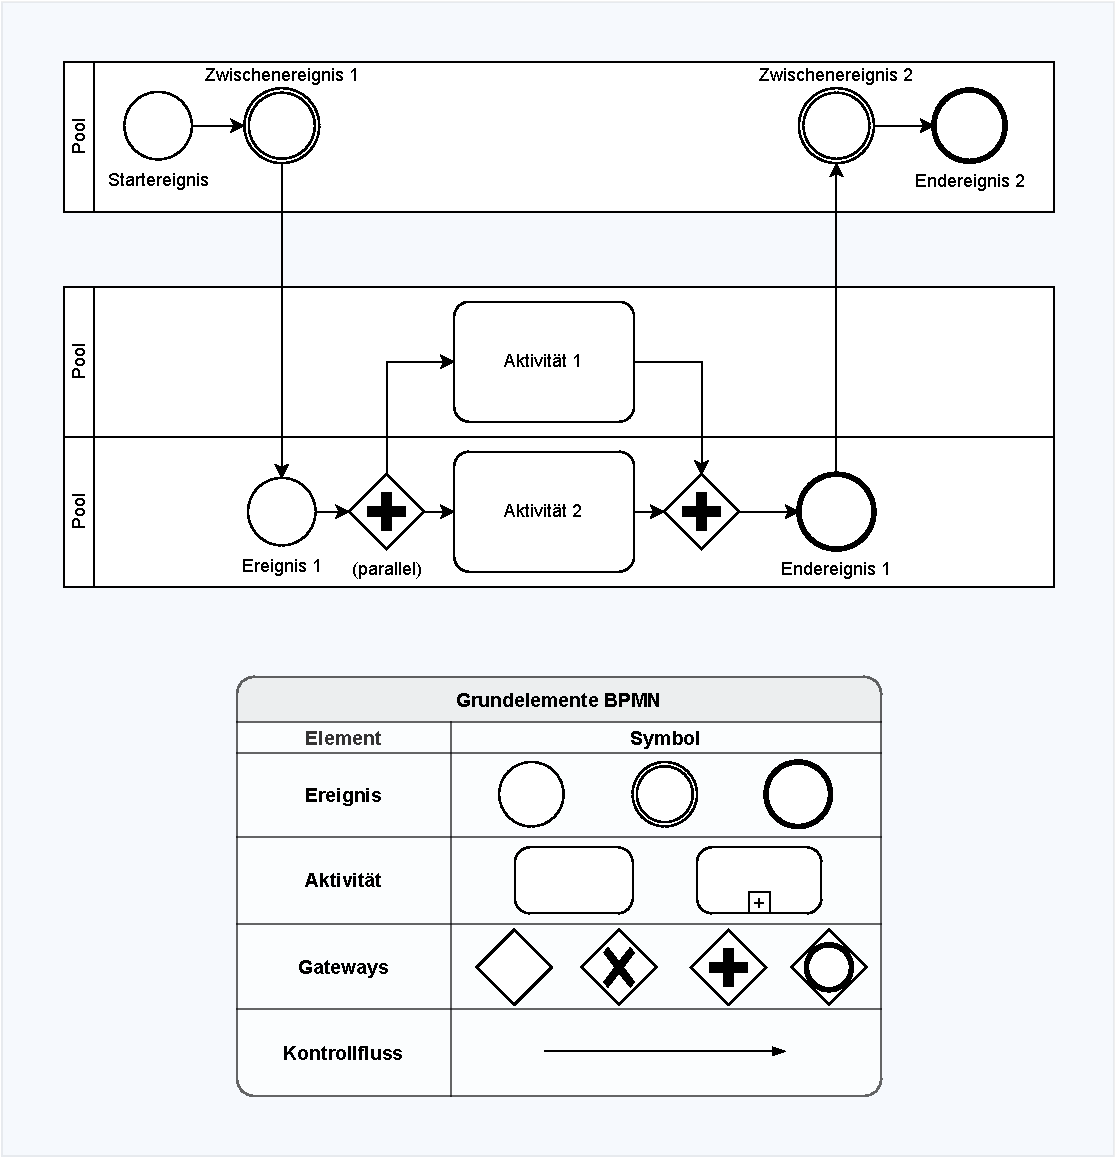
\includegraphics[scale=0.9]{Bilder/Kapitel-5/grundelemente_BPMN.pdf}
		\caption{BPMN}
		\label{fig:grundelemente_BPMN}
	\end{addmargin*}
	\end{addmargin*}
\end{figure}

BPMN bietet eine sehr große Palette an Symbolen, um Geschäftsprozesse detailliert abzubilden. Die zentralen Elemente sind allerdings auch hier Aktivitäten, lokale Zustände (wieder „Ereignisse“ genannt) sowie die Beschreibung des Kontrollflusses durch Pfeile und verschiedene Konnektoren.

\clearpage

\subsection*{Unterscheidung von System, Prozess und Ablauf}

Die Konzepte System, Prozess, Ablauf und weitere werden in der Literatur häufig verwendet, aber oft nicht hinreichend unterschieden. Bei einer formalen Modellierung mit Petrinetzen haben wir die Möglichkeit, diese Begriffe zu präzisieren.

Wenn wir von Realwelt-Modellierung sprechen, dann meinen wir nie die ganze Welt, sondern stets einen Ausschnitt. Wir müssen also festlegen, \textbf{was} wir modellieren wollen, und dabei auch, was nicht, und an welchen Stellen es relevante Schnittstellen gibt zwischen dem behandelten Ausschnitt und dem Rest. Dieser Schritt ist bereits eine erste Abstraktion: Wir abstrahieren von allem, was wir nicht betrachten wollen und reduzieren das gesamte relevante Verhalten dieser Restwelt zu Schnittstellen.


\begin{figure}[!htbp]
	\centering
	\resizebox{\textwidth}{!}{
		\begin{tikzpicture}
			\sffamily % kompletter Text ohne Serifen
			\bfseries % ... fett
			\Huge % ... und größer
			
			% Realwelt/Modell: Rechtecke mit abgerundeten Ecken und transparenter Füllung
			\fill[white!20!black, rounded corners=40pt, opacity=0.1] (-5,0) rectangle (15,20);
			\draw[white!20!black, thick, rounded corners=40pt] (-5,0) rectangle (15,20);
			\node[white!20!black, anchor=south east] at (1,18) {(Real-)Welt};
			
			\fill[FernUni-MI-green, rounded corners=40pt, opacity=0.2] (18,0) rectangle (38,20);
			\draw[FernUni-MI-green, thick, rounded corners=40pt] (18,0) rectangle (38,20);
			\node[FernUni-MI-green, anchor=south east] at (37,18) {Modell};
			
			% System/Systemmodell: Kreise
			%\fill[white, rounded corners=10pt] (5,13) circle (4.5);
			\fill[blue!30!black, rounded corners=10pt, opacity=0.2] (5,13) circle (4.5);
			\draw[blue!30!black, line width=0.5mm] (5,13) circle (4.5);
			\node[blue!30!black] at (5,15) {System};
			
			%\fill[white, rounded corners=10pt] (28,13) circle (4.5);
			\fill[blue!30!black, rounded corners=10pt, opacity=0.2] (28,13) circle (4.5);
			\draw[blue!30!black, line width=0.5mm] (28,13) circle (4.5);
			\node[blue!30!black] at (28,15) {Systemmodell};
			
			% Prozess/Prozessmodell: Rechtecke abgerundet
			\fill[white, rounded corners=15pt] (1.5,10.9) rectangle (8.5,12.1);
			\draw[rounded corners=15pt, line width=0.5mm] (1.5,10.9) rectangle (8.5,12.1);
			\node[] at (5,11.5) {Prozess};
			
			\fill[white, rounded corners=15pt] (24.5,10.9) rectangle (31.5,12.1);
			\draw[rounded corners=15pt, line width=0.5mm] (24.5,10.9) rectangle (31.5,12.1);
			\node[] at (28,11.5) {Prozessmodell};
			
			% Abläufe: Rechtecke abgerundet
			\fill[white] (7,6) rectangle (13.5,8);
			\draw[blue!30!black, line width=0.5mm] (7,6) rectangle (13.5,8);
			\node[blue!30!black] at (10.25,7) {Systemablauf};
			
			\fill[white] (19.5,6) rectangle (29.4,8);
			\draw[blue!30!black, line width=0.5mm] (19.5,6) rectangle (29.4,8);
			\node[blue!30!black] at (24.5,7) {Systemmodellablauf};
			
			\fill[white] (1.9,3) rectangle (8.3,5);
			\draw[line width=0.5mm] (1.9,3) rectangle (8.3,5);
			\node[] at (5,4) {Prozessablauf};
			
			\fill[white] (22.2,3) rectangle (32,5);
			\draw[line width=0.5mm] (22.2,3) rectangle (32,5);
			\node[] at (27.3,4) {Prozessmodellablauf};
			
			% Pfeile
			\draw[red,thick, ->, line width=2mm, -latex] (23.4,13) to (9.5,13);
			\draw[red,thick, ->, line width=2mm, -latex] (24.4,11.5) to (8.6,11.5); 
			\draw[red,thick, ->, line width=2mm, -latex] (19.4,7) to (13.5,7);
			\draw[red,thick, ->, line width=2mm, -latex] (22.1,4) to (8.3,4);
			
			% gestrichelte Linien
			\draw[dashed,blue!30!black, thick, -, line width=1.5mm] (24.7,9.9) to (23,8);
			\draw[dashed,blue!30!black, thick, -, line width=1.5mm] (8.3,9.9) to (10,8);
			\draw[dashed,black, thick, -, line width=1.5mm] (5,10.9) to (5,5);
			\draw[dashed,black, thick, -, line width=1.5mm] (30,10.9) to (30,5);
	\end{tikzpicture}}
	\caption{Modellierung von Systemen, Prozessen und Abläufen}
	\label{fig:v3-system_prozess}
\end{figure}


%Abbildung~\ref{fig:v3-system_prozess} zeigt...\\

Im ausgewählten Weltausschnitt, dem \textbf{System}, 
\marginline{System und Systemmodell}
gibt es vielfältige Aspekte, die mit Verhalten, also möglichen Veränderungen und dafür verantwortlichen Aktivitäten zu tun haben. Auf diese Aspekte konzentrieren wir uns bei der Verhaltensmodellierung, von anderen Aspekten abstrahieren wir. Auf Modellebene gilt es nun, das System zu modellieren mittels eines \textbf{Systemmodells}, in dem mit Elementen einer \textbf{Modellierungssprache} das relevante Systemverhalten nachgebildet wird.

Dieses Verhalten wird -- grob gesagt -- konstituiert durch die \textbf{Abläufe} des Systems. 
\marginline{Systemablauf, Aktivitäten und Aktionen}
Jeder \textbf{Systemablauf} stellt ein tatsächlich mögliches oder ein stattgefundenes Verhalten dar, definiert durch die \textbf{Aktivitäten}, die stattfinden. Wir nennen das Stattfinden einer Aktivität \textbf{Aktion}. Mehrere Aktionen eines Systemablaufs können sich auf dieselbe Aktivität beziehen, wenn diese mehrfach stattfindet. Zwischen den Aktionen eines Systemablaufs gibt es eine Abhängigkeitsbeziehung: Eine Aktion kann erst dann geschehen, wenn zuvor eine andere geschehen ist.

Das Systemmodell bildet das System dann korrekt ab, 
\marginline{Semantik bestimmt das Modellverhalten}
wenn man auch vom Modell Abläufe ableiten kann, die den Systemabläufen entsprechen, also als Modelle der Systemabläufe verstanden werden können. Während der Zusammenhang zwischen System und Systemablauf durch die Realität gegeben ist (im System können diese Abläufe geschehen), wird die Beziehung zwischen Systemmodell und seinen Abläufen durch die Semantik der Modellierungssprache definiert: Sie muss spezifizieren, was wir als Ablauf eines Systemmodells betrachten. Das Modellverhalten ist also nicht mit dem Modell selbst gegeben, sondern wird durch die Semantik passend konstruiert.

\vspace{1mm} %%% für Druck

\phantomsection
\label{text:prozesse_als_teilsysteme}
Auch wenn der Begriff System sehr umfassend ist, 
\marginline{Prozesse als Teilsysteme}
wollen wir nun zwei, im Bereich des Softwareengineering typische Klassen von Systemen genauer anschauen: Die erste, die wir im Folgenden einfach \textbf{Systeme} nennen werden, wird vielleicht durch die Beispiele Aufzugsteuerungssystem, Betriebssystem oder Datenbanksystem ganz gut charakterisiert. Im Softwareengineering aber schaut man insbesondere auch auf \textbf{Prozesse}, die von Systemen unterstützt oder generiert werden können. Formal betrachten wir einen Prozess auch als ein Teilsystem (und damit auch als System) eines größeren Systems. Daher gibt es auch Prozessmodelle, Prozessabläufe und Prozessmodellabläufe, und die Prozessabläufe sollen den Prozessmodellabläufen entsprechen.

\vspace{1mm} %%% für Druck

Typisch für Systeme ist, 
\marginline{(erwünschte) Eigenschaften von Systemen}
dass sie grundsätzlich immer weiter laufen können und nicht irgendwann aufgrund von gegenseitigem Warten verteilter Komponenten, Ressourcenmangel oder Ähnlichem steckenbleiben, also Zustände erreichen, in denen keine weiteren Aktivitäten mehr möglich sind (Deadlocks). Mehr noch, man wird von derartigen Systemen zusätzlich erwarten, dass es stets möglich ist, alle definierten Aktivitäten wieder auszuführen (ein Aufzugsteuerungssystem ist Deadlock-frei, auch wenn eine Etage irgendwann nie wieder erreicht werden kann, aber sicherlich nicht korrekt). Ein System mit dieser Eigenschaft heißt \textbf{lebendig}. Eine vermeint\-liche Möglichkeit, ein System lebendig zu halten, mag man darin sehen, beliebig viele neue Dokumente, Ressourcen, Aufträge, Nachrichten etc. zu generieren, sodass alle Systemkomponenten stets zu tun haben und nicht steckenbleiben. Derartige Systeme haben aber konsequenterweise eine unbeschränkte Menge erreichbarer Zustände, was sie erstens sehr unübersichtlich und unhandlich macht und zweitens ignoriert, dass in der Realität alle Speicher (in einem sehr allgemeinen Sinn) nur eine endliche Kapazität haben. Davon zu abstrahieren, führt schließlich auch zu Fehlern, wie man sie bei der Software-Erstellung kennt. Wir nennen derartige Systeme \textbf{unbeschränkt} und wünschen uns \textbf{beschränkte} Systeme. Deadlock-Freiheit, Lebendigkeit und Beschränktheit findet man als formale Qualitätskriterien wieder auf der Ebene von Systemmodellen.

\vspace{1mm} %%% für Druck

Die typischen Qualitätskriterien von Prozessen 
\marginline{(erwünschte) Eigenschaften von Prozessen}
unterscheiden sich deutlich von denen der Systeme. Zur Motivation dient das Beispiel des Aufzugsteuerungssystems. Wozu dient es? Es soll erlauben, dass jederzeit eine Person in irgendeiner Etage den Knopf drücken kann, irgendwann der Aufzug kommt, die Person einsteigt, in der Aufzugskabine ihr Ziel angibt ... und sie schließlich die gewünschte Etage erreicht. Andere typische Prozesse sind zum Beispiel bei dem System eines Versicherungsunternehmens die Abwicklung eines Schadens von der Schadensmeldung bis zur Auszahlung oder vom Versicherungsantrag bis zum fertigen Vertrag. Typischerweise ist mit einem Prozess ein Ziel verbunden, das irgendeinen Wert (für wen auch immer) hat. Wir erwarten, dass jeder Ablauf des Prozesses -- der durch ein Ereignis wie „Knopfdruck“, „Schadensmeldung“ oder „Versicherungsauftrag“ initiiert wird -- sein Ziel erreicht, wenigstens aber schließlich zu einem gewollten Ende kommt. Ein Prozess soll nicht lebendig oder Deadlock-frei sein, aber steckenbleiben oder unbeschränkte Ressourcen generieren soll er auch nicht. Wir werden später sehen, dass der Begriff „soundness“ auf Modellebene das gewünschte Verhalten von Prozessen ganz gut beschreibt.

\minisec{Definitionen der Begriffe}

\sttpDefinitionskasten{\sttpDefinitionskastenSkalierungsfaktorKapPN}{Definition 5.1: System}{}
{Ein System ist ein physisches oder logisches, existierendes oder gedachtes Regelwerk zu Ausführungen von Aktivitäten des Systems in einzelnen Abläufen.}

\vspace{-\baselineskip} % bei zwei aufeinanderfolgenden Definitionskästen Abstand verkleinern
\vspace{-2mm} % für Druck

\sttpDefinitionskasten{\sttpDefinitionskastenSkalierungsfaktorKapPN}{Definition 5.2: Systemablauf}{}
{Ein Systemablauf besteht aus Aktionen, die Instanzen (Stattfinden von) Aktivitäten sind, samt der kausalen Abhängigkeiten zwischen den Aktionen.}

\vspace{-\baselineskip} % bei zwei aufeinanderfolgenden Definitionskästen Abstand verkleinern
\vspace{-2mm} % für Druck

\sttpDefinitionskasten{\sttpDefinitionskastenSkalierungsfaktorKapPN}{Definition 5.3: Prozess}{}
{Ein Prozess ist ein Systemausschnitt, der eine Menge von Abläufen produzieren kann, welche von einem Startzustand zu einem Endzustand führen (sollen).}

\vspace{-\baselineskip} % bei zwei aufeinanderfolgenden Definitionskästen Abstand verkleinern
\vspace{-2mm} % für Druck

\sttpDefinitionskasten{\sttpDefinitionskastenSkalierungsfaktorKapPN}{Definition 5.4: Prozessablauf}{}
{Ein Prozessablauf ist die einmalige Durchführung eines Prozesses.}

\vspace{-\baselineskip} % für Druck

\subsection*{Verwendung der Modellierungssprachen im Softwareengineering}

Die bereits erwähnten Modellierungssprachen EPK und BPMN sowie UML-Akti\-vi\-täts\-dia\-gramme dienen der Modellierung von Prozessen und finden im Software\-engineering weite Verbreitung, insbesondere bei der Realwelt-Modellierung. Entsprechende Petrinetze sind Workflow-Petrinetze, die wir in den späteren Vorlesungen kennenlernen werden. An ganz anderer Stelle tauchen Verhaltensmodelle im Softwareengineering aber auch auf: Das Verhalten von Objekten, also ihre Zustands\-veränderungen und die Auslöser dafür, werden in Zustandsdiagrammen beschrieben (die diesen zugrundeliegenden State Charts (\cite{har87}) dienen allerdings auch der Realwelt-Modellierung). Wir können diese aber auch als spezielle (sequentielle) Petrinetze interpretieren. Schließlich hat sich für die Modellierung von Objekt\-interaktionen das UML-Sequenzdiagramm bewährt (auch diese Sprache hat ihren Ursprung in einem anderen Bereich, nämlich der Telekommunikation). Jedes derartige Diagramm hat viele Gemeinsamkeiten mit einem Petrinetz-Ablauf, also der Systemmodellablauf-Ebene. 
